\documentclass[border=3pt]{standalone}
% Preâmbulo compartilhado pelos diagramas TikZ da aula 10 de IHC (Planejamento da Avaliação)
\usepackage[T1]{fontenc}
\usepackage[utf8]{inputenc}
\usepackage{lmodern}
\usepackage{amsmath}
\usepackage{xcolor}
\usepackage{tikz}
\usetikzlibrary{arrows.meta,angles,quotes,decorations.pathmorphing,decorations.pathreplacing,calc,
                positioning,shapes.geometric,shapes.misc,backgrounds,fit,
                math}

% Paleta (mesma dos SVGs originais)
% Paleta da disciplina de IHC: acento roxo (#755099), da capa do livro.
% (o nome "dblue" é mantido para não alterar todos os diagramas)
\definecolor{dblue}{HTML}{755099}
\definecolor{dorange}{HTML}{B3541E}
\definecolor{dgreen}{HTML}{4A7C59}
\definecolor{dred}{HTML}{9C4B4B}
\definecolor{dcream}{HTML}{F4F1EA}
\definecolor{dshade}{HTML}{DDD7C9}

% Função gaussiana (não normalizada por padrão de escala visual)
\pgfmathdeclarefunction{gauss}{3}{%
  \pgfmathparse{1/(#3*sqrt(2*pi))*exp(-((#1-#2)^2)/(2*#3^2))}%
}

% Estilos comuns (prefixo d... para não colidir com chaves internas do pgf)
\tikzset{
  >={Stealth[length=2mm]},
  dguide/.style={gray!55, dashed, line width=0.4pt},
  daxis/.style={gray!60, line width=0.7pt, ->},
  dbody/.style={fill=black!3, draw=black!80, line width=1pt},
  dacc/.style={draw=dblue, line width=1pt},
  dlbl/.style={black!55, font=\small},
  dsub/.style={black!45, font=\footnotesize},
  dstate/.style={circle, draw=black!80, fill=dcream, line width=1pt,
                 minimum size=17mm, font=\large, inner sep=1pt},
  dobs/.style={circle, draw=black!80, fill=dshade, line width=1pt,
               minimum size=14mm, font=\large, inner sep=1pt},
  dbox/.style={rounded corners=2pt, draw=black!80, fill=dcream, line width=1pt,
               align=center, inner sep=6pt},
  dop/.style={circle, draw=black!80, fill=white, line width=1pt,
              minimum size=6mm, inner sep=0pt, font=\small},
  dtrans/.style={->, dblue, line width=1pt},
  dmeas/.style={->, dorange, line width=1pt},
  dcurve/.style={line width=1pt, dblue},
  dcurveb/.style={line width=1.4pt, dorange},
}

\begin{document}
\hyphenpenalty=10000 \exhyphenpenalty=10000 \tolerance=9999 \emergencystretch=3em
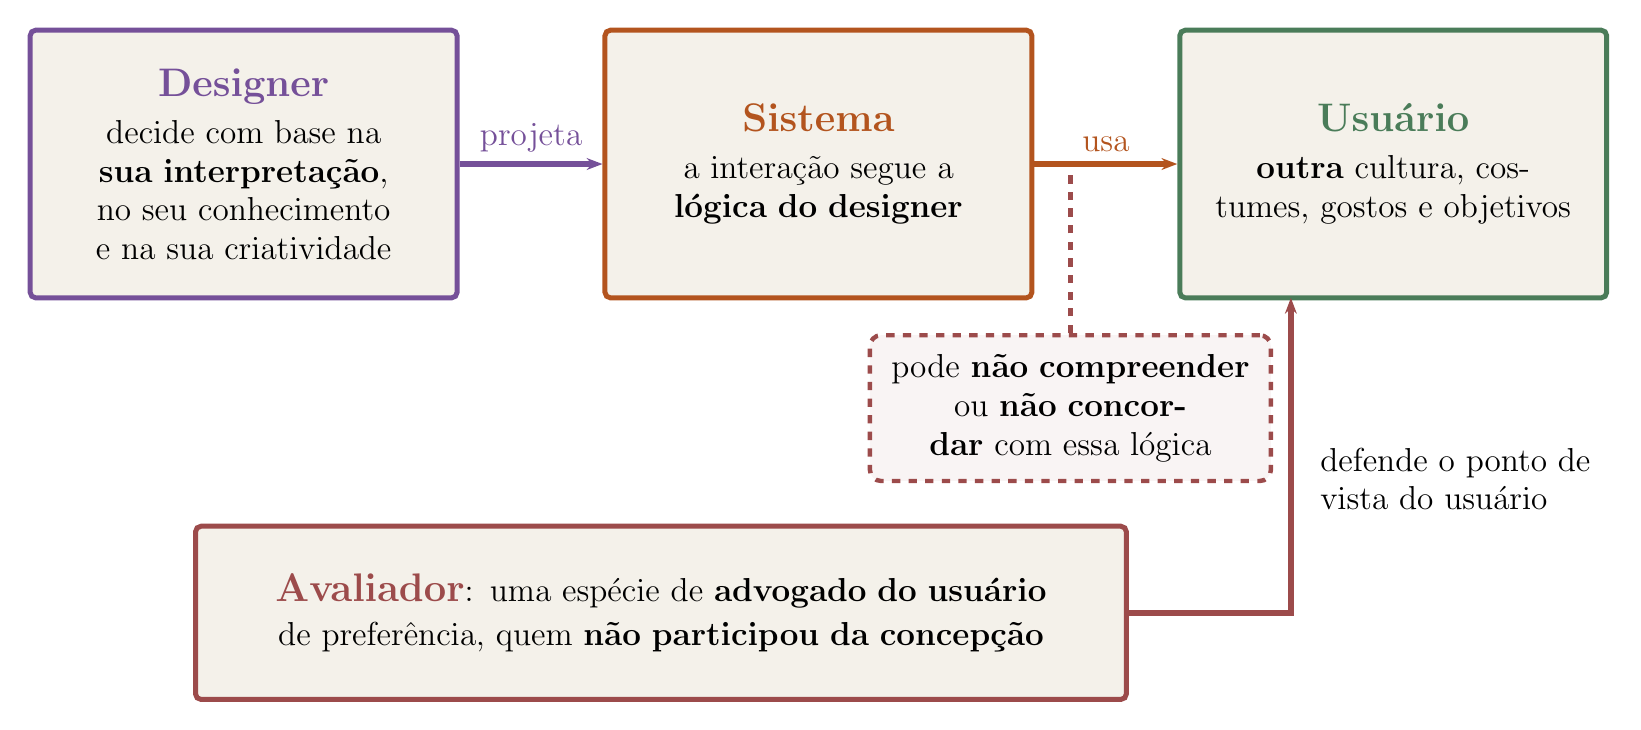
\begin{tikzpicture}[x=1cm,y=1cm]
\tikzset{k/.style={dbox, text width=5.0cm, minimum height=3.4cm, font=\large, line width=1.8pt}}
\node[k, draw=dblue] (d) at (2.7,5.4) {\textbf{\Large\textcolor{dblue}{Designer}}\\[3pt] decide com base na \textbf{sua interpretação}, no seu conhecimento e na sua criatividade};
\node[k, draw=dorange] (s) at (10.0,5.4) {\textbf{\Large\textcolor{dorange}{Sistema}}\\[3pt] a interação segue a \textbf{lógica do designer}};
\node[k, draw=dgreen] (u) at (17.3,5.4) {\textbf{\Large\textcolor{dgreen}{Usuário}}\\[3pt] \textbf{outra} cultura, costumes, gostos e objetivos};
\draw[->, line width=2.4pt, dblue] (d.east) -- node[above, font=\large] {projeta} (s.west);
\draw[->, line width=2.4pt, dorange] (s.east) -- node[above, font=\large] {usa} (u.west);
\node[draw=dred, dashed, line width=1.6pt, rounded corners=4pt, fill=dred!6, text width=4.6cm, align=center, font=\large, inner sep=7pt] (q) at (13.2,2.3) {pode \textbf{não compreender} ou \textbf{não concordar} com essa lógica};
\draw[dashed, line width=1.6pt, dred] (q.north) -- (13.2,5.35);
\node[dbox, draw=dred, text width=11.4cm, minimum height=2.2cm, font=\large, line width=1.8pt] (a) at (8.0,-0.3) {\textbf{\Large\textcolor{dred}{Avaliador}}: uma espécie de \textbf{advogado do usuário}\\[2pt] de preferência, quem \textbf{não participou da concepção}};
\draw[->, line width=2.4pt, dred] (a.east) -| (16.0,3.7);
\node[anchor=west, font=\large, text width=3.6cm, align=left] at (16.25,1.4) {defende o ponto de vista do usuário};
\end{tikzpicture}
\end{document}
